The H4 beamline will be extended to the NP04 cryostat, which houses ProtoDUNE-SP,  in the newly constructed extension of EHN1. To produce particles in the momentum range of interest, the 80-GeV/c pion beam from the T2 primary target is sent onto a secondary target to generate a tertiary beam. Particles in the tertiary beam are momentum- and charge-selected and transported down the H4 beamline extension to the detector. %into the protoDUNE-SP detector. 
In principle, the H4 beamline can operate in parallel with the H2 beamline, which will intercept the ProtoDUNE-DP detector, installed in the same building. The beamline layout is described and illustrated in Section~\ref{sec:h4beamline}. % minimize interference between the two ProtoDUNE experiments.

%%%%%%%%%%%%%%%%%%%%%%%%%%%%%%%%%%%%%%%%%%%%%%
\section{Beam requirements}
\label{sec:beamrequirements}

%The requested beam parameters are driven by the requirement that the results from the CERN test beam should be directly applicable to the future large underground single-phase LAr detector with minimal extrapolation. The CERN test beam data will be used to evaluate the detector performance, to understand the various physics systematic effects, and to provide data for event reconstruction studies that are representative of neutrino interactions. To satisfy the requirement, the beam parameters must span a broad range of particle momenta to match the charged particle spectrum and topologies that are expected in the DUNE far detector. The particle beam composition should consist of electrons, muons, and hadrons and needs to be charge-selected. The expected momentum distributions for secondary particles from neutrino interactions are shown in Figure~\ref{fig:particlemomenta}. There is a large spread in the momentum distribution with a clear peak near 200 MeV/c momentum per particle. The desirable momentum range for ProtoDUNE-SP  is in the low momentum region. Based on the feedback and constraints from the CERN beam group, the requested beamline design allows the transport of beam particles from about 0.5 GeV/c up to 7 GeV/c. 

The CERN test beam results from ProtoDUNE-SP will be used to evaluate the detector performance,  understand the various physics systematic effects, and provide data for event reconstruction studies that are representative of neutrino interactions. 
The parameters defining the test beam are primarily driven by the requirement that these test beam results be directly applicable to DUNE's future large underground single-phase detector module(s) with minimal extrapolation.
To match the charged-particle spectrum and topologies that are expected in the DUNE far detector, the beam must span a broad range of particle momenta, be composed of electrons, muons, and hadrons, and be charge-selected. \fixme{charge-selectable? Anne} 
The expected momentum distributions for secondary particles from neutrino interactions in the far detector, shown in Figure~\ref{fig:particlemomenta}, exhibit a large spread with a clear peak near 200~MeV/c per particle. \fixme{where is this figure?}
The desirable range for ProtoDUNE-SP is in the low-momentum region. Based on the feedback and constraints from the CERN beam group, the beamline design has been developed to allow the transport of beam particles from about 0.5~GeV/c up to 7~GeV/c. 
\fixme{it sounds like the CERN beam group is a different group than the one that designed the beamline. Is that right?}

The maximum electron drift time in the \fixme{ProtoDUNE-SP} TPC is about 2.25~ms. In order
to keep the  pile-up in the TPC at the percent level, the planned
beam particle rate should be about 100 Hz.  
\fixme{Is the beam not bunched? I guess I'm not used to ``particle rate''. Anne}
The ProtoDUNE-SP TPC has two drift volumes separated by a
passive cathode plane. It is desirable to aim the particle beam such
that a large fraction of the lower-energy hadronic showers are %mostly
contained in one drift volume, thus minimizing the uncertainties from
particles lost in the inactive detector materials. It is also
important to be able to inject beam into the cryostat at multiple
locations to study the detector
response. Figure~\ref{fig:beamwindow_loc} shows the three proposed
beam injection points.  The angles of the beam, with respect to the APA plane
are 3$^\circ$ (beam \#1), 8$^\circ$ (beam \#2), and 12$^\circ$ (beam
\#3). Due to engineering and safety considerations, only beam \#3 will
be fully instrumented with the beam window system as described in
Sections~\ref{subsec:beamwindow} and~\ref{sec:beamplug}. The remaining two beam positions will have
partial installation of the beam window system. With this
configuration, beam \#3 is the primary beam %where 
with which most of the physics
data will be taken.
\begin{cdrfigure}[Beam window locations]{beamwindow_loc}{Planned beam window locations.}
  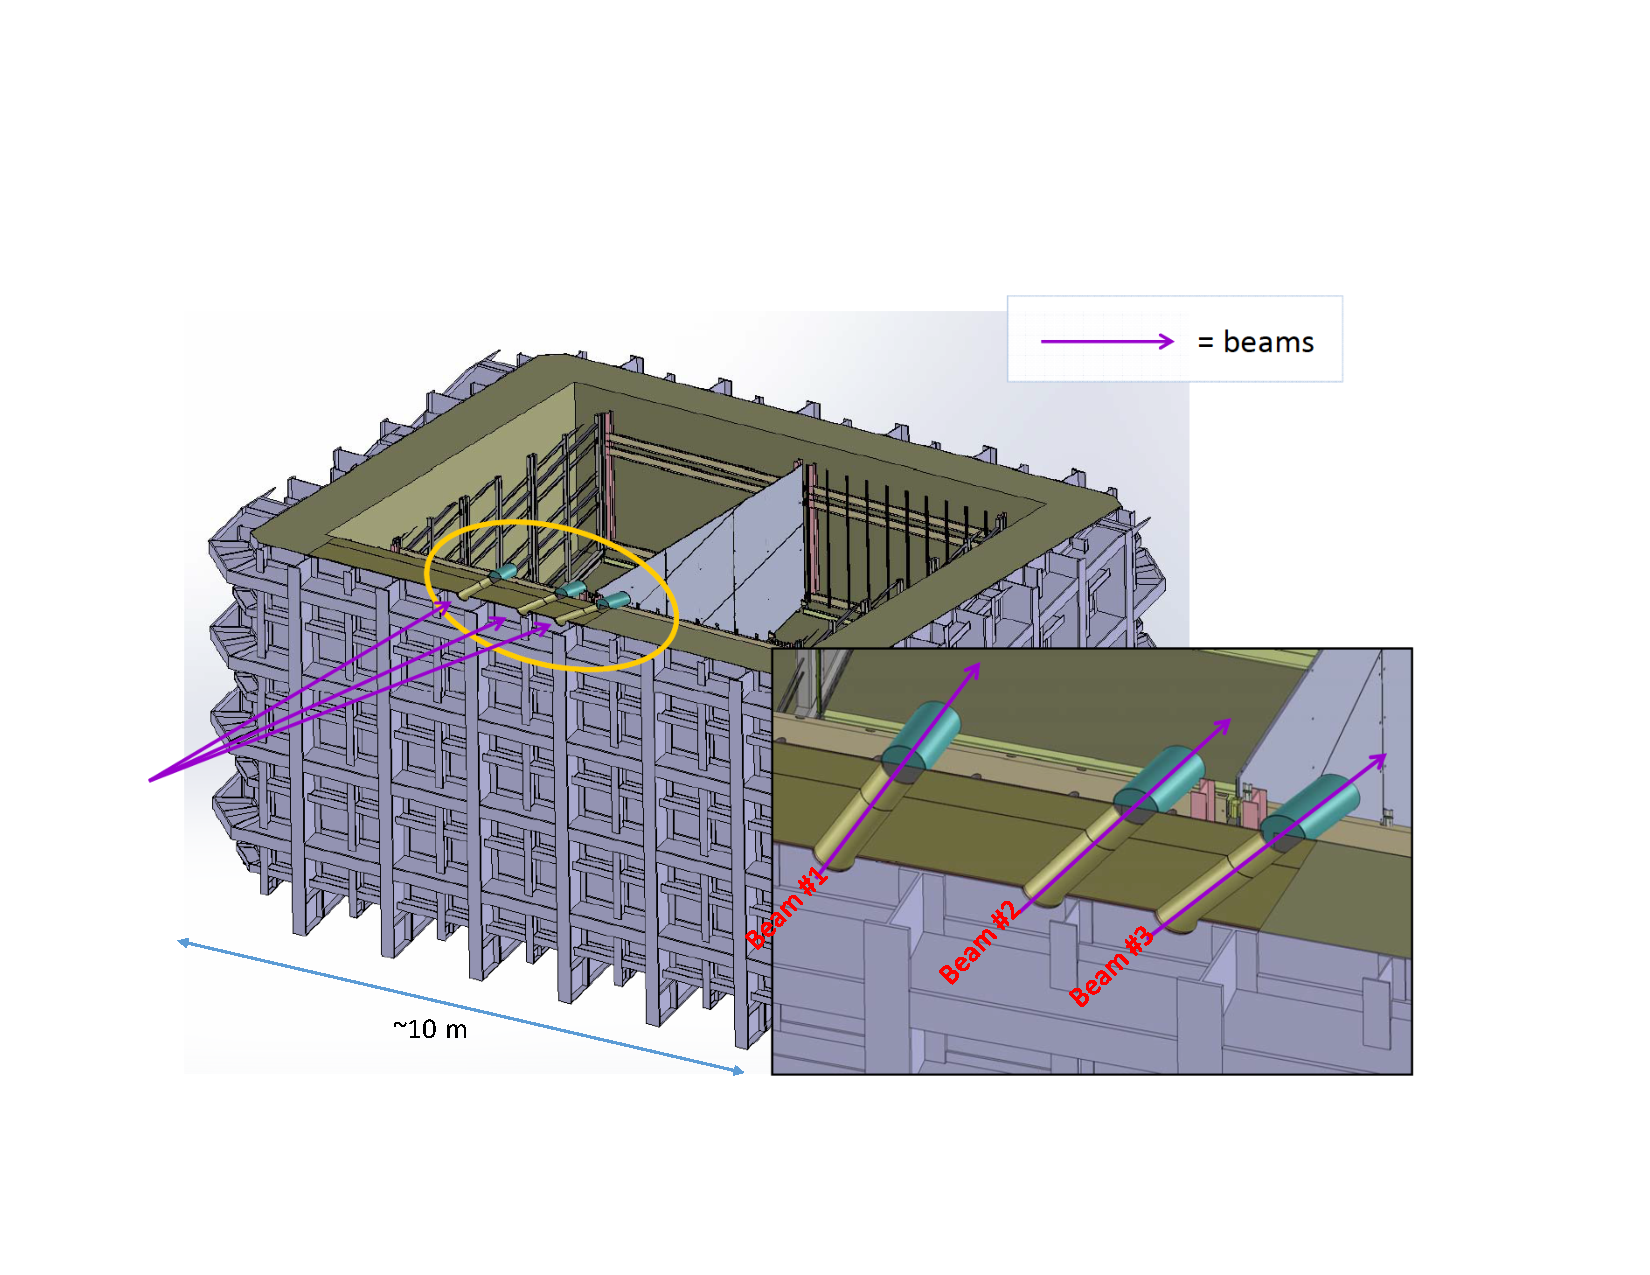
\includegraphics[width=0.9\textwidth]{beamwindow_locations.pdf}
\end{cdrfigure}
\fixme{ Although explained in the text, this figure with three equal beam penetrations/plugs is misleading, should be modified}
A summary of the beam requirements is shown in Table~\ref{tab:beamspecs}.
\begin{cdrtable}[Particle beam requirement]{ll}{beamspecs}{Particle beam requirements. (Kaon rate is low for beam momentum below 2 GeV/c.)}
%\textbf{Parameter } & \textbf{Requirements}  \\ \hline
 Parameter & Requirements \\ \toprowrule
  Particle Types        & $e^\pm,\mu^\pm,\pi^\pm$,$(K)$,$p$  \\ \colhline
  Momentum Range   & 0.5 - 7 GeV/$c$ \\ \colhline
  Momentum Resolution   & $\Delta p/p   \le 3$ \% \\ \colhline
  Transverse Beam Size   & RMS(x,y) $\approx$ 1 cm  \\
  & (At the entrance face of the LAr cryostat) \\ \colhline
%  Beam Divergence & tbd   \\ \colhline
  Beam Entrance Position & Multiple beam windows    \\ \colhline
  Rates & 25-$\approx$ 100 Hz     \\ \colhline
\end{cdrtable}

%\fixme{momentum spread/characterization: need tomato clear that this is w/o any beam monitor information}
\fixme{we should have beam divergence estimates from H2 and H4 simulation files Paola: again, the data from Nikos are a result,  NOT a requirement. If the physics or measurements group do have a requirement, please provide one! I took the line out, waiting for input.}
%\fixme{rate: max of 100 Hx; nominal 25Hz with goal to achieve 50 Hz (see CERN workshop)}
